\documentclass{article}[12pt]
\usepackage[catalan]{babel}
\usepackage[utf8]{inputenc}   % Permet usar tots els accents i car�ters llatins de forma directa.
\usepackage{enumerate}
\usepackage{amsfonts, amscd, amsmath, amssymb}
\usepackage[pdftex]{graphicx}
\usepackage{longtable}

\setlength{\textwidth}{16cm}
\setlength{\textheight}{24.5cm}
\setlength{\oddsidemargin}{-0.3cm}
\setlength{\evensidemargin}{0.25cm} \addtolength{\headheight}{\baselineskip}
\addtolength{\topmargin}{-3cm}

\newcommand\Z{\mathbb{Z}}
\newcommand\R{\mathbb{R}}
\newcommand\N{\mathbb{N}}
\newcommand\Q{\mathbb{Q}}
\newcommand\K{\Bbbk}
\newcommand\C{\mathbb{C}}
\newcommand\cT{{\cal T}}
\def\fl{\text{fl}}
\def\pt{\text{pt}}
\def\fm{\text{fm}}

\newcounter{exctr}
\newenvironment{exemple}
{ \stepcounter{exctr} 
\hspace{0.2cm} 
\textit{Exemple  \arabic{exctr}: }
\it
\begin{quotation}
}{\end{quotation}}

\pagestyle{empty}

\begin{document}

\begin{center}
\textbf{\Large Fonament i Aplicacions del Processament Digital dels Senyals \\ Grau de Telemàtica \\ Examen Setembre 2012}
\end{center}

\begin{description}

\item[Problema 1]. 

Donat l'esquema de la figura següent:

\begin{center}
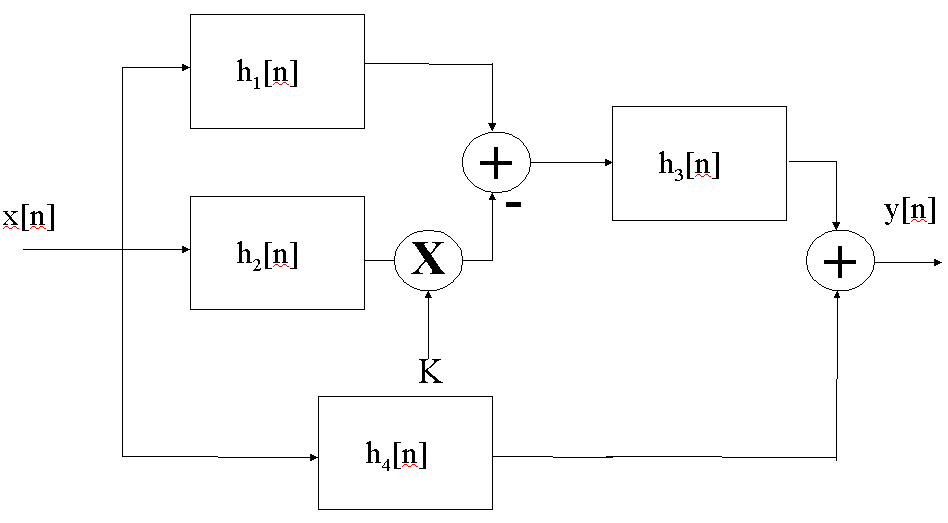
\includegraphics[width=10cm]{esquemaP1.png}
\end{center}

\noindent
on $h_1[n]=2 (\frac{1}{2})^n u[n]$, $h_2[n]=h_1[n-4]$, $h_3[n]=\{ \underline{-1}, 0, 1 \}$
i $h_4[n]=\{ \underline{a}, 0, b, 0, c, 0 \}$.

\vskip 0.3 cm
\noindent
Trobau els valors de les constants $K$, $a$, $b$ i $c$ que fan que el sistema es comporti com
un filtre FIR de fase lineal generalitzada de tipus IV.


\vskip 0.5cm


\item[Problema 2].

Considerau un sistema LTI causal IIR recursiu definit per la següent equació:
\[
y[n]-y[n-1]+4y[n-2]-4y[n-3]=x[n]-\frac{1}{4}x[n-2]
\]

\begin{enumerate}[a)]
\item Dibuixau les formes directa i canònica del sistema.
\item Calculau la funció de transferència del sistema $H(z)$.
\item Dibuixau el diagrama de zeros i pols i justificau si el sistema és estable o no.
\item Calculau la resposta impulsional del sistema $h[n]$.
\end{enumerate}  


\vskip 0.5cm


\item[Problema 3].

La següent figura representa el mòdul de la DFT d'un senyal digital $x[n]$,
obtingut per discretització amb $N=55000$ mostres d'un senyal continu,
amb una freqüència de mostreig $F_s=11025$ Hz.

\begin{center}
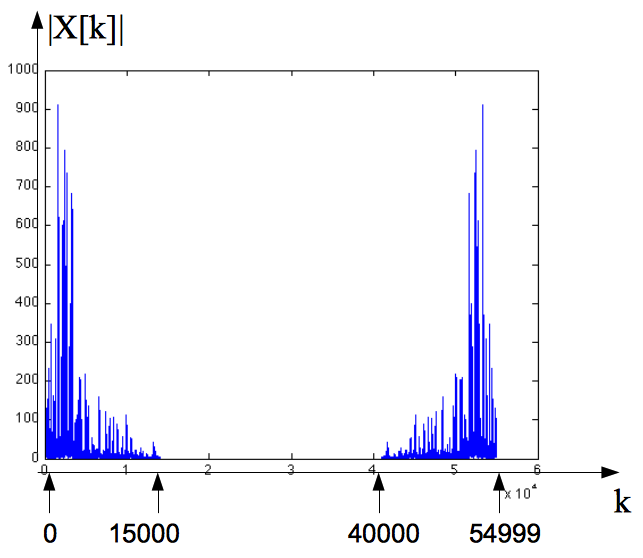
\includegraphics[width=10cm]{fftP3b.png}
\end{center}

\begin{enumerate}[a)]
\item Pensau que $x[n]$ és un senyal real? Per què?
\item Pensau que s'ha produit aliasing quan s'ha mostrejat el senyal continu? Per què?
\item Pensau que es podria submostrejar $x[n]$ amb un factor de submostreig 2
(és a dir, obtenir $x_{subm}[n]=x[2n]$) sense que es produís aliasing? Per què?
\item A quin rang de freqüències contínues (en Hz)  corresponen els valors de $X[k]$ compresos entre $k=6000$ i $k=8000$?
\item Quina és l'amplada de banda del senyal (la freqüència contínua, en Hz, major que conté el senyal)?
\item Si volguèssim eliminar la component espectral amb freqüència contínua (aproximada) $900$ Hz, per a quins
valors de $k$ hauriem de fer $X[k]=0$?
\item Si reconstruïm el senyal amb una freqüència de mostreig doble de l'original obtindrem un senyal
de sortida més ràpid o més lent que l'original? Justificau la resposta.
\item Si reconstruïm el senyal amb una freqüència de mostreig doble de l'original l'amplada de banda del
senyal de sortida serà major o menor que l'original? Justificau la resposta.
\end{enumerate}  

\vskip 0.5cm


\item[Problema 4].

Volem dissenyar un filtre FIR causal real de fase lineal amb el menor nombre de mostres possible que atenui totalment les freqüències discretes $\omega=\pi/4$ i $\omega=0$ (és a dir $X(\omega)=0$ per a $\omega=\pi/4$ i $\omega=0$).

\begin{enumerate}[a)]
\item Dibuixau el diagrama de zeros i pols del filtre.
\item Calculau la funció de transferència $H(z)$ del filtre.
\item Calculau la resposta freqüencial $H(\omega)$ del filtre i calculau la seva fase.
\item Calculau la resposta impulsional $h[n]$ del filtre i digau de quin tipus de filtre FIR es tracta (I, II, III o IV).
\item Calculau la resposta del filtre al senyal d'entrada $x[n]=\{\underline{-1}, 0, 1\}$.
\end{enumerate}


\end{description}

\vskip 2cm

\noindent
Duració de l'examen: 4 hores.



\end{document}
